%%% Hlavní soubor. Zde se definují základní parametry a odkazuje se na ostatní části. %%%

%% Verze pro jednostranný tisk:
% Okraje: levý 40mm, pravý 25mm, horní a dolní 25mm
% (ale pozor, LaTeX si sám přidává 1in)
%\documentclass[12pt,a4paper]{report}
%\setlength\textwidth{145mm}
%\setlength\textheight{247mm}
%\setlength\oddsidemargin{15mm}
%\setlength\evensidemargin{15mm}
%\setlength\topmargin{0mm}
%\setlength\headsep{0mm}
%\setlength\headheight{0mm}
%% \openright zařídí, aby následující text začínal na pravé straně knihy
%\let\openright=\clearpage

%% Pokud tiskneme oboustranně:
 \documentclass[12pt,a4paper,twoside,openright]{report}
 \setlength\textwidth{145mm}
 \setlength\textheight{247mm}
 \setlength\oddsidemargin{14.2mm}
 \setlength\evensidemargin{0mm}
 \setlength\topmargin{0mm}
 \setlength\headsep{0mm}
 \setlength\headheight{0mm}
 \let\openright=\cleardoublepage

%% Vytváříme PDF/A-2u
\usepackage[a-2u]{pdfx}

%% Přepneme na českou sazbu a fonty Latin Modern
\usepackage[czech]{babel}
\usepackage{lmodern}
\usepackage[T1]{fontenc}
\usepackage{textcomp}

%% Použité kódování znaků: obvykle latin2, cp1250 nebo utf8:
\usepackage[utf8]{inputenc}

%%% Další užitečné balíčky (jsou součástí běžných distribucí LaTeXu)
\usepackage{amsmath}        % rozšíření pro sazbu matematiky
\usepackage{amsfonts}       % matematické fonty
\usepackage{amsthm}         % sazba vět, definic apod.
%\usepackage{bbding}         % balíček s nejrůznějšími symboly
			    % (čtverečky, hvězdičky, tužtičky, nůžtičky, ...)
\usepackage{bm}             % tučné symboly (příkaz \bm)
\usepackage{graphicx}       % vkládání obrázků
\usepackage{fancyvrb}       % vylepšené prostředí pro strojové písmo
\usepackage{indentfirst}    % zavede odsazení 1. odstavce kapitoly
%\usepackage{natbib}         % zajištuje možnost odkazovat na literaturu
			    % stylem AUTOR (ROK), resp. AUTOR [ČÍSLO]
\usepackage[nottoc]{tocbibind} % zajistí přidání seznamu literatury,
                            % obrázků a tabulek do obsahu
\usepackage{icomma}         % inteligetní čárka v matematickém módu
\usepackage{dcolumn}        % lepší zarovnání sloupců v tabulkách
\usepackage{booktabs}       % lepší vodorovné linky v tabulkách
\usepackage{paralist}       % lepší enumerate a itemize
\usepackage[usenames]{xcolor}  % barevná sazba

%%% Údaje o práci

% Název práce v jazyce práce (přesně podle zadání)
\def\NazevPrace{Plánovač spojení ve městě}

% Název práce v angličtině
\def\NazevPraceEN{Urban transport planner}

% Jméno autora
\def\AutorPrace{Tomáš Pokorný}

% Rok odevzdání
\def\RokOdevzdani{2017}

% Název katedry nebo ústavu, kde byla práce oficiálně zadána
% (dle Organizační struktury MFF UK, případně plný název pracoviště mimo MFF)
\def\Katedra{Katedra aplikované matematiky}
\def\KatedraEN{Department of Applied Mathematics}

% Jedná se o katedru (department) nebo o ústav (institute)?
\def\TypPracoviste{Katedra}
\def\TypPracovisteEN{Department}

% Vedoucí práce: Jméno a příjmení s~tituly
\def\Vedouci{Mgr. Martin Mareš, Ph.D.}

% Pracoviště vedoucího (opět dle Organizační struktury MFF)
\def\KatedraVedouciho{Katedra aplikované matematiky}
\def\KatedraVedoucihoEN{Department of Applied Mathematics}

% Studijní program a obor
\def\StudijniProgram{Informatika}
\def\StudijniObor{Diskrétní modely a algoritmy}

% Nepovinné poděkování (vedoucímu práce, konzultantovi, tomu, kdo
% zapůjčil software, literaturu apod.)
\def\Podekovani{%
Na tomto místě bych rád poděkoval Mgr. Martinu Marešovi, Ph.D. za cenné rady a
odbornou pomoc při konzultacích k~této práci. Dále bych rád poděkoval svým
kamarádům a speciálně Ing. Petru Pechovi za podporu a motivaci při psaní práce.
Také bych rád poděkoval Anetě Šťastné za pomoc s~finální úpravou práce.
}

% Abstrakt (doporučený rozsah cca 80-200 slov; nejedná se o zadání práce)
\def\Abstrakt{%
Cestování po městě je součástí každodenního života mnoha lidí. Zvolit správnou
kombinaci pěší chůze a cestování hromadnou dopravou bývá náročné, obzvlášť
v~neznámých částech města. Zpracovali jsme veřejně dostupná data a vytvořili
vyhledávač kombinovaných tras pěšky a hromadnou dopravou. Vyhledávač byl navržen
s~důrazem na možnost přizpůsobit hledané trasy preferencím uživatelů a lze jej
použit i jako webovou aplikaci nebo sdílenou knihovnu.
}
\def\AbstraktEN{%
Travelling in the city is a part of everyday life for many people. It is
sometimes difficult to choose the right combination of walking and public
transport especially in unfamiliar parts of the city. We processed publicly
available data and made a search engine for multimodal paths. The search engine
was designed to be able to personalise results according to user needs and could
be used as a web application or a shared library.
}

% 3 až 5 klíčových slov (doporučeno), každé uzavřeno ve složených závorkách
\def\KlicovaSlova{%
{vyhledávač spojení} {jízdní řád} {penalta} 
}
\def\KlicovaSlovaEN{%
{multimodal search engine} {timetable} {penalty}
}

%% Balíček hyperref, kterým jdou vyrábět klikací odkazy v PDF,
%% ale hlavně ho používáme k uložení metadat do PDF (včetně obsahu).
%% Většinu nastavítek přednastaví balíček pdfx.
\hypersetup{unicode}
\hypersetup{breaklinks=true}

%% Definice různých užitečných maker (viz popis uvnitř souboru)
\include{makra}

%% Titulní strana a různé povinné informační strany
\begin{document}
\include{titulka}

%%% Strana s automaticky generovaným obsahem diplomové práce

\tableofcontents

\newcommand{\TODO}{\textcolor{red}{TODO:}}

%%% Jednotlivé kapitoly práce jsou pro přehlednost uloženy v samostatných souborech
\chapwithtoc{Úvod}

Hledání cesty ve městě je častou situací většiny lidí. Ve městě se vyskytuje
mnoho různých překážek jako jsou ploty, zábradlí či frekventované silnice,
i mnoho průchozích prostranství, například náměstí, parky či sady. V naší práci
se snažíme z mapových dat vytvořit formát vhodný pro rychlé vyhledávání pěších
tras využívajících i průchozí prostranství. Tato práce by měla být jedním z~modulů
budoucí aplikace pro vyhledávání spojení pěšky a MHD po městě. 

%\section{Co chci počítat}
Abychom mohli rychle vyhledávat pěší trasy, potřebujeme k~tomu mít mapu vhodně
reprezentovanou. Vstupní mapová data postupně zpracováváme a vybíráme z nich
použitelné informace. Na konci tohoto procesu vytvoříme graf popisující možné
pěší trasy. V tomto grafu již můžeme vyhledávat pomocí grafových algoritmů pro
hledání cest, v ukázkové aplikaci využíváme Dijkstrův algoritmus. 

%\section{Zdroje dat}
Abychom mohli vyhledávat trasy, potřebujeme k~tomu vhodné mapové podklady.
Protože jsme chtěli, aby bylo možné zpracovaná data volně používat a šířit, 
potřebovali jsme získat i takové mapové podklady. Proto jsme si vybrali jako
zdroj dat OpenStreetMap (OSM), volně dostupné mapové podklady vytvářené komunitou. 
Projekt OpenStreetMap využívá k~tvorbě mapy mimo práce dobrovolníků také jiné
volně dostupné mapové podklady a poskytuje pravěpodobně nejlepší veřejně
dostupná mapová data. Jako zdroj dat o~nadmořské výšce jsme použili data
z~projektu SRTM, která jsou také volně dostupná.

%\section{Co už kdo napsal}
K~porovnání výsledků naší aplikace jsme použili nejznámější webové mapové
aplikace -- Google Maps a Mapy.cz. Také jsme nalezené trasy porovnávali s~jinými
vyhledávači používajícími data OSM -- OsmAnd a TODO. Nalezené trasy jsme také
porovnávali s~vlastní znalostí terénu a skutečně používaných cest.

%TODO: obrazek - vstupni data a vystupni data

\chapter{Rešerše}
Data o různých cestních sítích obvykle ukládáme ve formě grafu, ve kterém pak
vyhledáváme jednotlivé trasy pomocí prohledávání grafu, na které existuje mnoho
známých algoritmů. Pokud ale potřebujeme udržovat kromě dat o cestní síti data o
jízdních řádech, stává se situace mnohem složitější, protože zatímco po cestách
můžeme jít kdykoli, cestovat hromadnou dopravou můžeme pouze tehdy, když zrovna
jede nějaký spoj. Pro reprezentaci sítí hromadné dopravy se vyvinuly různé
způsoby, dále představíme nejobvyklejší z nich.

\section{Time-dependent modely}
Time-dependent modely \cite{time-dependent} se snaží odstranit problém s
velikostí grafu hromadné dopravy. Místo toho, abychom měli pro každý spoj
zvláštní hranu, sdružíme spoje do linek, kde všechny spoje jedné linky mají
stejnou posloupnost zastávek. Vrcholy tentokrát budou jen jeden pro každou
zastávku. Hrany mezi zastávkami budou jedna pro každou linku, která danou
dvojici zastávek spojuje. V takovémto grafu již nemůžeme vyhledávat pomocí
běžného průchodu grafu, potřebujeme mít upravenou funkci, která vyhledá v
jednotlivých časech odjezdu pro každou linku nejbližší od okamžiku příjezdu do
zastávky. Tento přístup nevytváří grafy s velkým počtem vrcholů a hran, navíc je
tato reprezentace snáze připojitelná do vyhledávacího grafu pro obyčejnou cestní
síť. U této varianty také existuje varianta, která má jeden staniční vrchol a
pro každou linku projíždějící danou stanicí linkový vrchol. Tyto vrcholy jsou
pak propojeny přestupovými hranami a umožňují realističtější modelování
rozsáhlejších stanic a přestupů v rámci nich. Ani tento model však nevyužívá
všech vlastností spojů MHD, jako je například to, že spoj má danou trasu a že
když na něj někde nastoupíme, tak snadno můžeme do fronty přidat všechny
průjezdní stanice.  

\section{Time expanded modely}
Time-expanded modely \cite{time-expanded} jsou konstruovány tak, aby ceny hran
byly konstantní a šlo na takovýto graf použít běžné vyhledávání v grafu. V
těchto modelech jsou jako vrcholy dvojice (zastávka, čas odjezdu) a (zastávka,
čas příjezdu) pro každý čas odjezdu a příjezdu z každé zastávky. Hrany pak
jsou jednak \uv{spojové} spojující vždy dvojici odjezd-příjezd mezi dvěma
zastávkami pomocí nějakého spoje, jednak \uv{čekací}, které spojují jednotlivé
časy v rámci jedné zastávky tak, jak jde čas. Spojení pak hledáme tak, že na
množině vrcholů patřících k výchozí zastávce najdeme vrchol s nejbližším vyšším
časem, než je náš odjezdový. Běžným průchodem do šířky podle času přes spojové a
čekací hrany pak najdeme cestu do cílové zastávky. Nevýhodou této reprezentace
je velikost grafu.

Tento základní model nerespektuje časy potřebné pro přestup, což může být
zvlášť problematické u rozsáhlých stanic či zastávek s mnoha zastávkovými
stojany. Tento problém se dá vyřešit rozdělením linie událostí u jedné zastávky
na více. Vrcholy patřící k jedné zastávce rozdělíme na zastávkové, příjezdové a
odjezdové. Odjezdové vrcholy odpovídají odjezdům spojů ze zastávky a příjezdové
vrcholy příjezdům do zastávky. Zastávkové vrcholy odpovídají každý jednomu
odjezdovému vrcholu. Zastávkové vrcholy jsou spojeny hranami do posloupnosti
stejně jako v původním grafu. Z příjezdového vrcholu vedou hrany do nejbližšího
zastávkového vrcholu, do kterého se stihne pěší přesun a do všech dřívějších
odjezdových vrcholů, do kterých se stihne pěší přesun. Ze zastávkového vrcholu
vede navíc hrana do odpovídajícího odjezdového vrcholu. 
\TODO obrázek
\section{Contraction hierarchy}
\section{RAPTOR}
RAPTOR (Round-Based Public Transport Routing) \citep*{RAPTOR} je oproti
time-dependent modelům založen na zcela odlišných myšlenkách a při svém běhu
nevyužívá Dijkstrův algoritmus. RAPTOR se snaží využít co nejvíce vlastností,
kterými se odlišuje síť veřejné dopravy od obyčejné cestní sítě. Také umožňuje
snadno optimalizovat na počet přestupů.

Algoritmus pracuje po kolech. Každé kolo zanmená nástup do dalšího dopravního
prostředku, celkově je tedy počet kol o 1 větší než maximální počet přestupů.
Algoritmus pracuje s linkami. Každá linka má několik spojů, což jsou konkrétní
vozidla, která všechna projíždí stejnou posloupnost zastávek. Každý spoj má
uloženy časy odjezdu z jednotlivých zastávek, předpokládáme, že se dva spoje
jedné linky na trase nepředjíždí. Pro každou zastávku si pro každé kolo
pamatujeme, zda a kdy je dosažitelná pomocí kterého kola. Nedosažitelnost
zastávky reprezentujeme pomocí nastavení času příjezdu v daném kole na $\infty$.

Na začátku jsou všechny zastávky ve všech kolech nedosažitelné. Nastavíme
výchozí zastávce čas dosažení v prvním kole na zadaný čas odjezdu a spustíme
algoritmus. Ten postupně prochzí linky po jejich zastávkách a pokud narazí na
dosažitelnou zastávku, tak najde nejbližší spoj linky, který z dané zastávky
odjíždí po čase dosažitelnosti a tímto spojem se \uv{vydá} a průběžně upravuje
časy dosažitelnosti na dalších zastávkách. Pokud po cestě nalezne další
dosažitelnou zastávku, jako spoj z této zastávky vybere ten z původního spoje a
spoje navazujícího na původní čas dosažitelnosti, který odjíždí dříve a takto
pokračuje až do konce linky. Po průchodu všech linek se všechny časy
dosažitelnosti zkopírují do dalšího kola a algoritmus se znovu spustí. Po
stanoveném počtu kol algoritmus skončí a u jednotlivých zastávek je pro každé
kolo (odpovídající počtu přestupů - 1) uloženo, zda je s daným počtem přestupů
dosažitelná a v jakém čase. K jednotlivým časům u zastávek je vhodné si uložit
ilinku, která způsobila úpravu na daný čas, abychom byli schopni zrekonstruovat
spojení využité k dosažení dané zastávky. 

Tento algoritus je snadno implementovatelný a při vhodně zvolených datových
strukturách velmi rychlý a vhodně využívající keš. 

\subsection{Uložení dat}
Pro rychlý výpočet a efektivní využití cache je potřeba mít vhodně uložená data.
Data stejného typu jsou vždy uložená v poli za sebou. Pokud různé objekty mají
každý mít seznam stejného typu, jsou všechna data od všech objektů držena v
jednom poli a každý objekt si drží počet svých prvků a odkaz na první z nich.
Tímto má každý objekt vyhrazen svůj úsek a může s ním efektivně pracovat. Tento
mechanismus nazveme \uv{polním mechanismem} a budeme na něj takto odkazovat ve
zbytku kapitoly.

Základem pro prohledávání je pole linek. Každá linka má odkaz na své zastávky a
na časy zastavení spojů v zastávkách. Obojí je implementováno polním mechanismem
a rozdělení na zastávky a spoje zajišťuje snadnou možnost hledání spojů v daný
čas. Časy zastavení spojů v zastávkách jsou uspořádány v poli za sebou podle
zastávek a pak podle času výjezdu spoje z výchozí zastávky. Protože
předpokládáme, že se spoje nepředjíždí a všechny spoje jedné linky mají stejný
počet zastávek, na předchozí spoj snadno přejdeme skokem v poli zastavení o
počet zastávek linky vzad, následující spoj najdeme obdobným skokem vpřed. Také
je možné pro konkrétní zastávku a konkrétní čas použít jednoduše binární
vyhledávání pro nalezení nejbližšího spoje odjíždějícího po konkrétním čase. 

Pro vyhledávání z konkrétní zastávky máme obdobně implementovány datové
struktury kolem zastávek. Zastávky jsou uloženy v poli za sebou, každá si drží
seznam linek, které jí projíždějí, a seznam pěších přestupů z dané zastávky. 
Obojí je reprezentováno polním mechanismem.   


\chapter{Zdrojová data}

Zdrojová data pro vyhledávač pochází ze dvou zdrojů. Prvním zdrojem jsou mapová
data, která obsahují silnice, cesty, budovy a další mapové prvky. Druhým zdrojem
jsou data o jízdních řádech, která obsahují linky, zastávky a spoje.

\section{Mapová data}
Mapová data jsou použita z projektu OpenStreetMap\cite{OSM} (OSM). Tato data neobsahují
informace o nadmořské výšce jednotlivých bodů; k doplnění nadmořské výšky jsou
použita data z projektu NASA Shuttle Radar Topography Mission (SRTM), která jsou
lineárně interpolována pro získání nadmořských výšek jednotlivých bodů v mapě.

O datech OSM a jejich problémech jsme již rozsáhle pojednávali v bakalářské
práci\cite{bakalarka}, níže citujeme obecný úvod a popis základních primitiv. 
\newcommand{\tuc}{\bf}
\subsection{Projekt OpenStreetMap}
Projekt OpenStreetMap\cite{OSM} vznikl v~Anglii v~roce 2004 a jeho prvotním cílem bylo
vytvořit volně dostupná geografická data pro Velkou Británii. Iniciativa se
postupně rozrostla do celého světa a dnes mapu pomáhá tvořit přes milion
dobrovolníků. Česká republika je dnes poměrně kvalitně pokryta a zvláště velká
města mají dostatečně detailní pokrytí i pro vyhledávání pěších tras.

\subsection{Datová primitiva OSM} 
Projekt OpenStreetMap používá tři základní geografická primitiva: uzly, cesty a
relace. Ke každému z~těchto primitiv mohou být přiřazeny atributy, což jsou
dvojice klíče a hodnoty. Každý typ primitiv má svou číselnou řadu, ze které
dostává každý prvek unikátní číslo -- id. 
U~polohových dat se neukládá výška, výsledná mapa je pouze dvourozměrná.
Nyní popíšeme jednotlivá primitiva:

{\tuc Uzly} jsou body s~určenými souřadnicemi. Uzly mohou mít atributy, ty pak
určují bodový mapový objekt, například rozcestník nebo závoru. Existují i uzly
bez atributů sloužící pouze jako součást cest nebo relací.

{\tuc Cesty} jsou lomené čáry definované posloupností uzlů. Uzly se na cestě nemohou opakovat
s~jedinou výjimkou: první a poslední bod mohou být shodné, potom se jedná
o~uzavřenou cestu. Cesty jsou orientované, tzn. na pořadí uzlů záleží. Mohou
existovat cesty bez atributů jako součásti relace, ale obvykle mají atributy
určující, jaký objekt reálného světa popisují.

Pomocí cest popisujeme linie a plochy. Pokud má být cesta plochou, musí být
uzavřená, ale ne každá uzavřená cesta je plocha. Tento problém rozebíráme níže.
Jedna cesta také může reprezentovat více fyzických objektů (například silnici
s~tramvajovou tratí, park s~oplocením).

{\tuc Relace} jsou posloupnosti uzlů a cest opatřené atributy. Každý prvek
v~relaci navíc může mít určenou roli. Relace může obsahovat jako prvek i relaci,
ale tato situace není příliš dobře podporována programy pracujícími s~daty OSM. 
Obvykle jsou relacemi reprezentovány složitější objekty, které by se cestami a
uzly popisovaly obtížně, nebo také \uv{virtuální} objekty jako například
trasy linek MHD, cyklotrasy a územní hranice.

Pro nás důležitý typ relace je {\tuc multipolygon}, který se používá k~reprezentaci
složitějších ploch. Plocha reprezentovaná multipolygonem se může skládat z~více
nesouvisejících částí nebo obsahovat díry. Multipolygon obsahuje cesty s~rolemi 
\verb|INNER| resp. \verb|OUTER| indikující, zda je cesta součástí vnější resp.
vnitřní hranice plochy. Hranice multipolygonu se mohou skládat z~více částí, ale
vždy musí dohromady tvořit jednu nebo několik uzavřených částí tvořících obvody 
plochy resp. díry v~ploše.

\section{Výšková data}
O výškových datech jsme také pojednávali v bakalářské práci, opět
citujeme\cite{bakalarka}:
Abychom mohli správně odhadnout náročnost pěší trasy, musíme znát i informace
o~nadmořské výšce jednotlivých bodů. Stejně tak jako většina jiných projektů jsme
použili data SRTM\cite{SRTM}, což jsou volně dostupná výšková data pro celý
svět.

Shuttle Radar Topography Mission byl projekt NASA, kdy při letu raketoplánu
Endeavour v~roce 2000 byla pomocí radarové interferometrie změřena velká část
Země a zpracovaná data byla následně poskytnuta volně k~dispozici.\footnote{\url{http://dds.cr.usgs.gov/srtm/version2_1/}} 

Výšková data byla měřena po třech úhlových vteřinách (v~USA po jedné vteřině),
tudíž v~České republice jsou data v~mřížce $90\times60$\,m. Data jsou rozdělena
do tabulek po jednom stupni, přičemž sousední tabulky se vždy jedním sloupcem
nebo řádkem překrývají. Každá tabulka má tedy 1201 sloupců a 1201 řádků, kde
řádky odpovídají zeměpisné šířce a sloupce zeměpisné délce.

Nadmořské výšky jsou kódovány celými 16bitovými čísly v~big endian udávajícími
nadmořskou výšku v~metrech. Pokud se v~některém místě nepodařilo výšku změřit,
je udávána jako $-32768$. Tabulka je kódována jako binární soubor, v~němž jsou
jednotlivé řádky zapsány za sebou.

\section{Jízdní řády}
Data o jízdních řádech jsou očekávána ve formátu General Transit Feed
Specification (GTFS) \cite{GTFS}, který je dobře specifikovaný a široce používaný ve světě.
Konkrétně pro testování byla použita data o pražské integrované dopravě od IPR
Praha.\footnote{\url{http://opendata.iprpraha.cz/DPP/JR/jrdata.zip}} Tato data
obsahují metro, tramvaje, autobusy a přívozy v Praze a okolí, bohužel neobsahují
integrované vlakové spoje.

GTFS je distribuováno jako archiv ZIP obsahující jednotlivé tabulky ve formátu
CSV. Význam jednotlivých tabulek je následující:
\begin{itemize}
\item {\em agency.txt} obsahuje informace o dopravcích na jednotlivých linkách.
V našem vyhledávání není používán.
\item {\em stops.txt} obsahuje informace o zastávkách. Zastávky jsou dvou typů.
Prvním typem je zastávkový stojan, který reprezentuje fyzické místo, kde
zastavuje nějaký spoj některé linky. Druhým typem je \uv{stanice}, která udává
oblast několika stojanů, obvykle stejného jména. Nemusí mít fyzickou
reprezentaci a slouží pro zobrazování v mapě a svázání logicky blízkých stojanů.
Protože stanice pro náš vyhledávač nenese důležitou informaci, využíváme pouze
zastávkové stojany. Pro vyhledávání spojení využíváme
následující položky:
\begin{itemize}
	\item {\tt stop\_id} -- jednoznačný identifikátor zastávky
	\item {\tt stop\_name} -- název zastávky
	\item {\tt stop\_lat, stop\_lon} -- poloha zastávky
	\item {\tt location\_type} -- informace, zda jde o stojan, nebo stanici
\end{itemize}
\item {\em routes.txt} obsahuje informace o linkovém vedení. Pro vyhledávání
spojení využíváme následující položky:
\begin{itemize}
	\item {\tt route\_id} -- jednoznačný identifikátor linky
	\item {\tt route\_short\_name} -- krátký název linky, v Praze označení linky
	\item {\tt route\_type} -- typ dopravního prostředku linky, například autobus, loď, metro
\end{itemize}
\item {\em trips.txt} obsahuje informace o spojích. Tato tabulka slouží ke
svázání spoje (cesty konkrétního dopravního prostředku po posloupnosti zastávek
v daný čas), linky a množiny dní, kdy daný spoj jezdí. Pro vyhledávání využíváme
následující položky:
\begin{itemize}
	\item {\tt route\_id} -- identifikátor linky
	\item {\tt service\_id} -- identifikátor jízdních dní spoje
	\item {\tt trip\_id} -- jednoznačný identifikátor spoje
\end{itemize}
\item {\em stop\_times.txt} obsahuje informace o časech zastavení jednotlivých
spojů v jednotlivých zastávkách. Pro vyhledávání spojení používáme následující
položky:
\begin{itemize}
	\item {\tt trip\_id} -- identifikátor spoje
	\item {\tt arrival\_time} -- čas příjezdu spoje do zastávky 
	\item {\tt departure\_time} -- čas odjezdu spoje ze zastávky
	\item {\tt stop\_id} -- identifikátor zastávky
	\item {\tt stop\_sequence} -- pořadí zastávky na spoji. Je potřeba, aby
	bylo nezáporné, celočíselné a po trase spoje se zvyšovalo, zvyšování po
	1 ani počítání od 0 není nutné.
\end{itemize}
\item {\em calendar.txt} obsahuje informace o tom, které dny v týdnu jezdí které
spoje. Pro vyhledávání spojení používáme následující položky:
\begin{itemize}
	\item {\tt service\_id} -- identifikátor jízdních dní spoje
	\item {\tt monday \dots{} sunday} -- informace, zda spoj jede daný den. 
	\item {\tt start\_date} -- první den platnosti jízdního řádu pro daný
	spoj
	\item {\tt end\_date} -- poslední den platnosti jízdního řádu pro daný
	spoj (tento den ještě v rámci platnosti).
\end{itemize}
\item {\em calendar\_dates.txt} obshauje výjimky z pravidelnosti spojů,
například státní svátky či jiná omezení. Obsahuje změny oproti souboru {\tt
calendar.txt}. Může být použit i samostatně bez souboru {\tt
calendar.txt}, pak obsahuje všechny jízdní dny daného spoje. Pro vyhledávání
spojení používáme následující položky:
\begin{itemize}
	\item {\tt service\_id} -- identifikátor jízdních dní spoje 
	\item {\tt date} -- datum změny
	\item {\tt exception\_type} -- typ změny (1 = jede navíc, 2 = nejede, ač
	by měl)
\end{itemize}
\end{itemize}


\chapter{Předzpracování dat}


\section{Příprava mapových dat}
Nejprve jsou stažena aktuální data pro Českou republiku, která jsou k~dispozici
s~denními aktualizacemi.\footnote{\url{osm.kyblsoft.cz/archiv/}} Z~těchto dat je
na základě nastavení vyříznut obdélník, který pokrývá zpracovávanou oblast. Poté
začneme data zpracovávat.

Nejprve jsou klasifikovány jednotlivé objekty. Klasifikují se uzly, hrany a
multipolygony, jiné typy relací nejsou v~současné době používány. Každý objekt
je klasifikován nějakým typem podle toho, jaké má tagy. V~rámci konfigurace lze
přidělit nějakému tagu (buď samotnému klíči, nebo dvojici klíč-hodnota) určený
typ s~danou prioritou. Objekt bude mít typ daný pravidlem s~nejvyšší prioritou,
které jeho tagy splňují. Pokud objekt nesplňuje žádné pravidlo, získá speciální
typ označující neklasifikovaný objekt.V dalším zpracování se již nehledí na
původní tagy ale jen na typ, který daný objekt má.

Současně s~klasifikací typu objektu se stejným způsobem určují hrany, které se
nachází na mostech a uzly, které jsou v~podzemí. Klasifikovaná data nahrajeme do
databáze a další kroky provádíme jako databázové operace. 

\subsection{Dělení dlouhých linií}
Protože chceme hledat co nejblíže od výchozího zadaného bodu, v~případě dlouhých
rovných ulic, které jsou reprezentovány pomocí lomených linií s~dlouhými úseky
by se nám mohlo stát, že by nejbližší bod od hledaného místa neležel na ulici,
kde jsme, ale na nějaké sousední, od které nás dělí pás budov. Proto dlouhé
úseky cest rozdělíme na menší podúseky (viz obr. \ref{fig:deleni}, čímž tento problém eliminujeme.
Rozdělení se nám také bude hodit pro vytváření zkratek, o~kterých pojednáváme
níže.

\begin{figure}
  \centering
    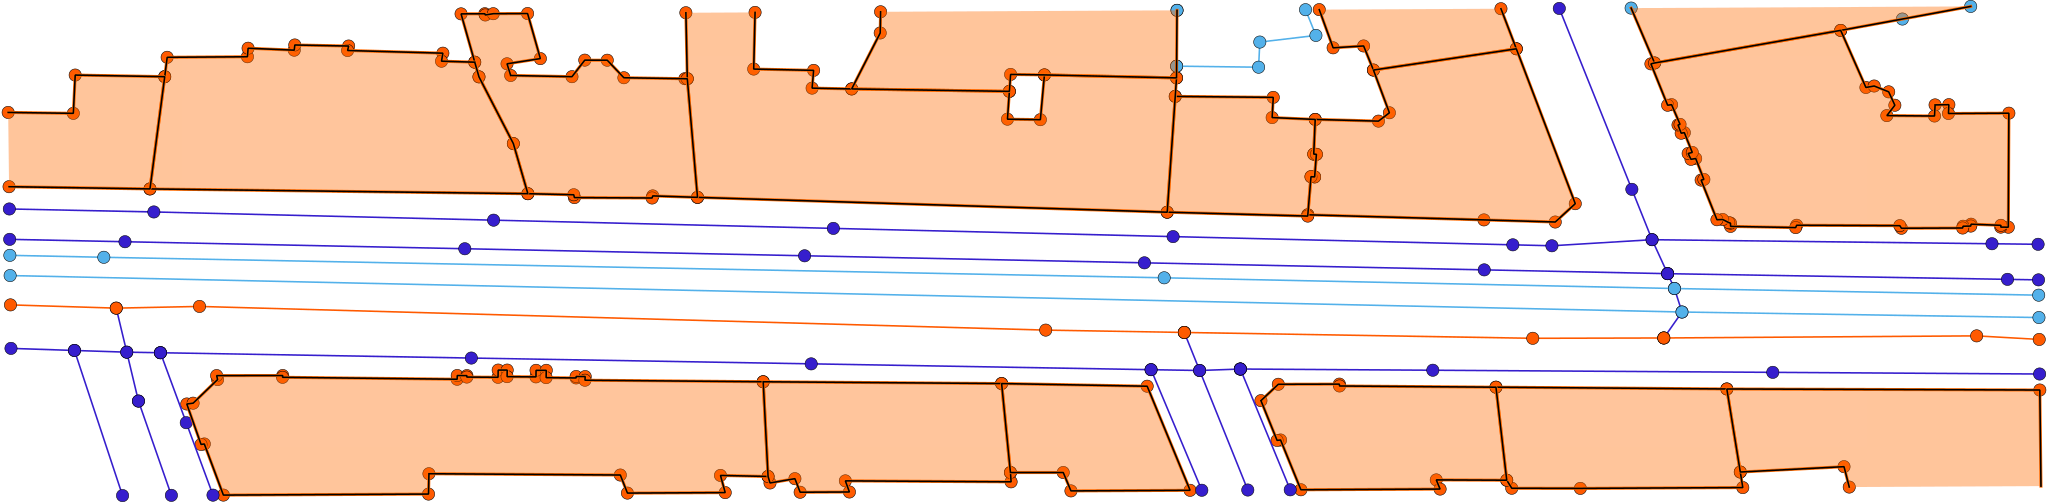
\includegraphics[width=0.75\textwidth]{../img/deleni.pdf}
  \caption{Rozdělení dlouhých linií (všimněte si, že jsou děleny jen pochozí
  linie)}
  \label{fig:deleni}
\end{figure}

\subsection{Překážky}
Pro další zpracování potřebujeme znát nejen cestní síť, ale i překážky, přes
které se nedá projít, jako jsou například domy, ploty a dálnice. V~tomto místě
se musíme vypořádat s~multipolygony. Protože multipolygony, které klasifikujeme
jako bariéry, jsou většinou budovy, které mají více částí nebo mají nádvoří,
nebo jiné překážky, uvnitř kterých neočekáváme velkou plochu, bereme
jako překážku jejich vnější obrys, případně obrysy. To nám sice způsobí, že
nebudeme moci vytvářet na vnitřních prostranstvích zkratky, ale to nám nevadí,
protože jednak mají vnitřní prostranství obvykle velmi malou plochu a nevede do
nich mnoho pěších cest, jednak vnitřní prostranství jsou buď zmapována
kompletně, nebo nedostatečně, tudíž by případné vytváření zkratek ve vnitřním
prostranství vedlo k~cestám, které by ve skutečnosti nebyly možné.

Výsledná množina překážek bude obsahovat vnější obrysy multipolygonů, další
polygonové objekty a liniové objekty.

\subsection{Body uvnitř objektů a body pod zemí}
Abychom mohli generovat zkratky, které budou průchozí i ve skutečnosti, je
potřeba určit, které body se nachází na volném prostranství na povrchu a které
se nacházejí pod zemí. Podzemní vrcholy jsme určili už v~rámci klasifikace.
Vrcholy uvnitř objektů jsme ztotožnili s~vrcholy, které se nachází uvnitř nějaké
překážky, protože překážky jsou pro nás takové objekty, přes které se nedá pěšky
projít napříč. Body, které se nacházejí na plášti překážky, jako vnitřní
neuvažujeme, protože se z~nich dá jít libovolným směrem, kde se nenachází
překážka.

\subsection{Zkratky}
Pro doplnění chybějících vazeb v~mapě používáme kromě cest v~mapových datech
již obsažených i automaticky generované zkratky. Zkratka spojuje dva pochozí
body na volném prostranství, které jsou nedaleko od sebe a úsečka mezi nimi,
reprezentující zkratku, neprotíná žádnou překážku. Dvojic bodů, které splňují
zadané podmínky, je ale velké množství a přidání všech zkratek by neúměrně
zvyšovalo velikost výsledných dat. Od počtu zkratek z~daného vrcholu přidávání
dalších zkratek má jen malý vliv na délky hledaných cest, proto jsou ze všech
možných zkratek náhodně vybrány jen některé a to tak, aby z~každého vrcholu
vycházelo průměrně omezené množství zkratek. Takto zachováme pozitivní vliv
zkratek na hledané cesty, ale zbytečně nezvětšujeme vyhledávací graf.
\begin{figure}
  \centering
    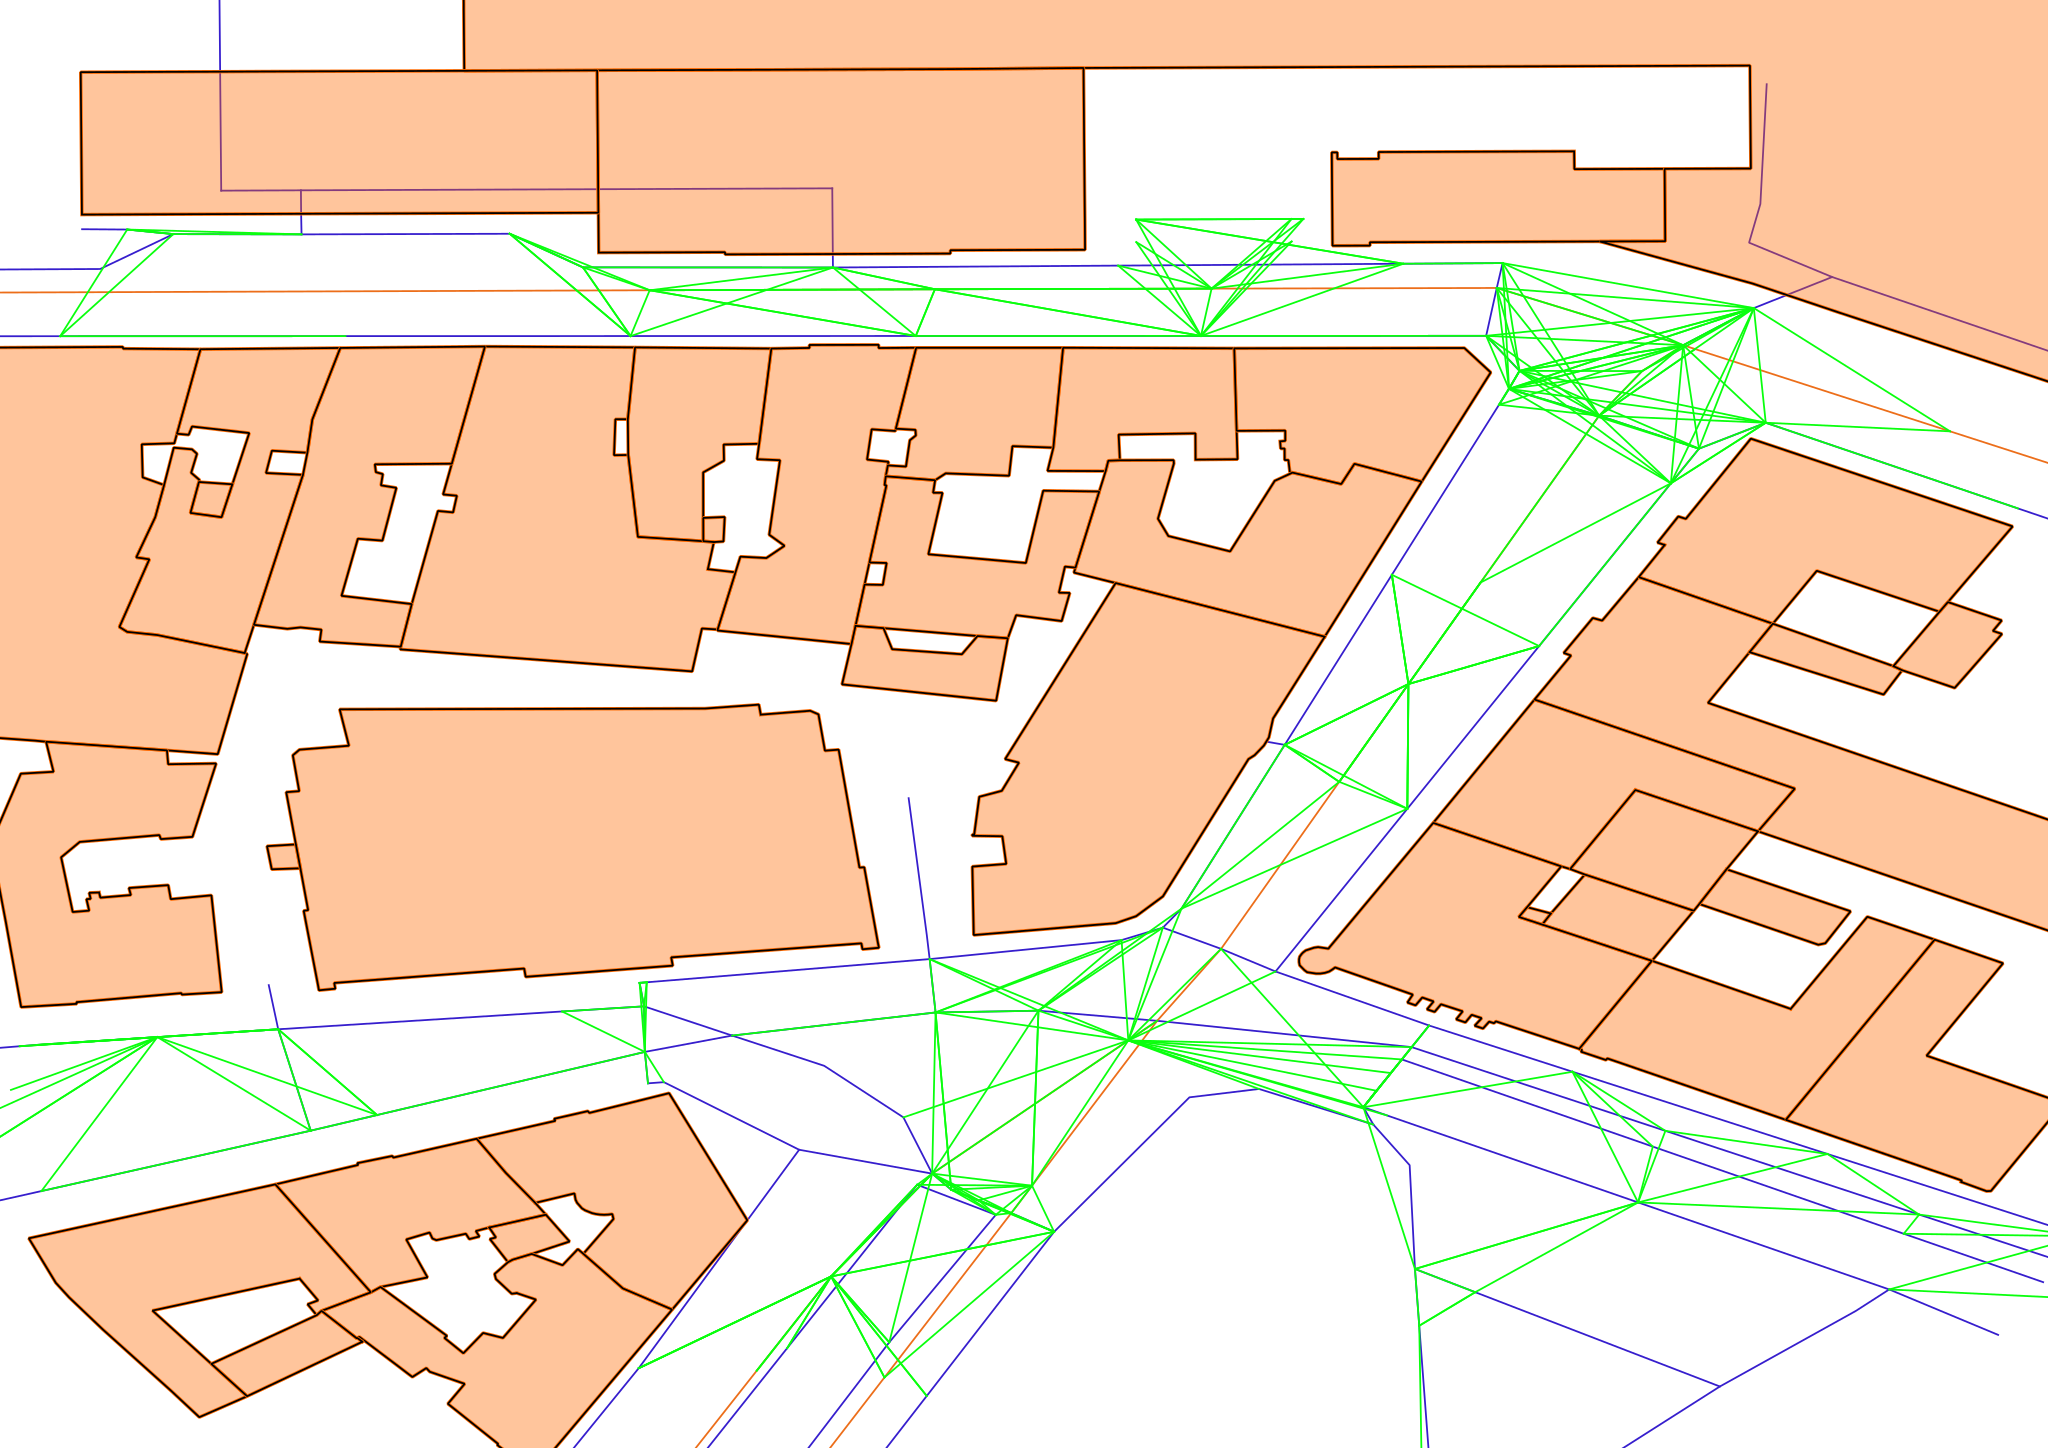
\includegraphics[width=0.5\textwidth]{../img/zkratky.pdf}
  \caption{Vygenerované zkratky mezi cestami (zeleně)}
  \label{fig:zkratky}
\end{figure}

\section{Příprava jízdních řádů}
Data z~jízdních řádů dostáváme ve formátu GTFS \cite{GTFS} a musíme je
upravit do formátu vhodného pro algoritmus RAPTOR \cite{RAPTOR}. V~rámci převodu
mezi formáty je potřeba respektovat specifické požadavky algoritmu RAPTOR a také
je potřeba připravit si informace potřebné pro propojení mezi zastávkami
v~jízdním řádu a zastávkami na mapě.

\subsection{Rozdělení linek}
Formát GTFS rozlišuje linky a spoje. Linka obsahuje všechny společné údaje a
jednotlivé spoje pak reprezentují jízdu vozidla dané linky mezi konkrétními
stanicemi, různé spoje jedné linky mohou projíždět různé posloupnosti stanic
(například spoje zatahující do vozovny, zkrácené vložené spoje, \dots).
Algoritmus RAPTOR ale vyžaduje, aby spoje konkrétní linky projížděly vždy
stejnou posloupnost zastávek. Abychom toho dosáhli, v~rámci předzpracování
najdeme všechny různé posloupnosti zastávek projížděné jednou linkou a vytvoříme
sublinky pro každou takovou posloupnost. Tyto sublinky zdědí společné údaje
z~původní linky a již splňují požadavky kladené algoritmem RAPTOR. 

\subsection{ID zastávek}
Zastávky mají dle specifikace GTFS jako ID použit obecný string. Data pro
pražskou MHD mají toto ID rozdělené na na část reprezentující zastávku a část
reprezentující konkrétní zastávkové stojany. Pro další zpracování je vhodné
zvolit číselný identifikátor, jednotlivé zastávky jsou očíslovány čísly od 0 do
počet zastávek $- 1$ a veškeré odkazy na konkrétní zastávky ve zpracovaných datech
používají právě tato čísla. Původní identifikátor je u~zastávky stále uložen
kvůli následnému párování (viz níže), ale již se pro vazbu mezi daty nepoužívá.

\subsection{Platnost jízdního řádu}
Ve formátu GTFS jsou linky, spoje a dny, ve kterých daný spoj jede, provázány
pomocí tabulky trips. V~předchozím odstavci jsme popsali rozdělení linek podle
toho, kudy spoje jedou, nyní využijeme, že každý spoj v~GTFS má právě jednu
množinu dní, kdy jede a tuto informaci si uložíme i u~jednotlivých spojů v~nově
vytvářeném formátu.

Místo dvojího způsobu záznamu, kdy daný spoj jede -- pomocí výčtu dnů v~týdnu a
seznamu výjimek -- si pro každou možnost, jak může nějaký spoj jet, uložíme
bitmapu platnosti a datum začátku a konce platnosti současného jízdního řádu. 
Bitmapa začíná první den platnosti a $i$-tý bit udává, zda i-tý den od začátku
platnosti daný spoj jede.  

\subsection{Podzemní stanice}
Při párování zastávek a pozic na mapě budeme potřebovat zvlášť ošetřovat
podzemní stanice, ze kterých se nelze vydat libovolným směrem, ale jen
eskalátorovým tunelem. V~rámci předzpracování označíme jako podzemní takové
zastávky, ve kterých jezdí metro. V~Praze takovýto předpoklad funguje správně,
protože všechny nadzemní stanice metra jsou zmapovány detailním způsobem, kdy
zpracování dat funguje korektně, pro jiná města s~jinou kvalitou zmapování by
bylo potřeba stanovit odlišná kritéria.


\section{Párování zdrojových dat}
Abychom moli plánovat spojení využívající jak pěší chůzi, tak jízdu MHD, je
potřeba data z~obou zdrojů vhodně provázat. Máme k~dispozici následující údaje:
\begin{enumerate}
\item OSM
\begin{itemize}
	\item jméno zastávky
	\item pozici zastávky
	\item ID zastávky (jen u~některých)
\end{itemize}
\item GTFS
\begin{itemize}
	\item jméno zastávky
	\item pozici zastávky
	\item ID zastávky
\end{itemize}
\end{enumerate} 
V~ideální případe by bylo možné spárovat zastávky jednoduše dle ID, bohužel
v~OSM má ID jen několik zastávek, většinu zastávek je tedy potřeba spárovat jinak.
Nabízelo by se párování podle pozic a jmen zastávek, ale bohužel zastávky v~GTFS
jsou výrazně posunuté oproti OSM i skutečnosti, navíc ne všechny zastávkové
stojany jsou v~OSM vyznačeny, zvláště tam, kde je několik zastávkových stojanů
za sebou, například v~autobusových terminálech. Pokoušet se párovat zastávky
v~GTFS pouze na zastávky v~OSM by bylo velmi náročné s~nejistým výsledkem.
Využíváme proto toho, že v~OSM máme zmapované nejen zastávky, ale i cesty a
zastávkám v~GTFS vytváříme speciální vrcholy dle jejich zeměpisné pozice v~GTFS
a pomocí zkratek je spojujeme s~nejbližšími cestami (viz Obrázek
\ref{fig:zastavka}. Bod reprezentující zastávku pak v~mapových datech označíme
jako zastávku.

\begin{figure}
  \centering
    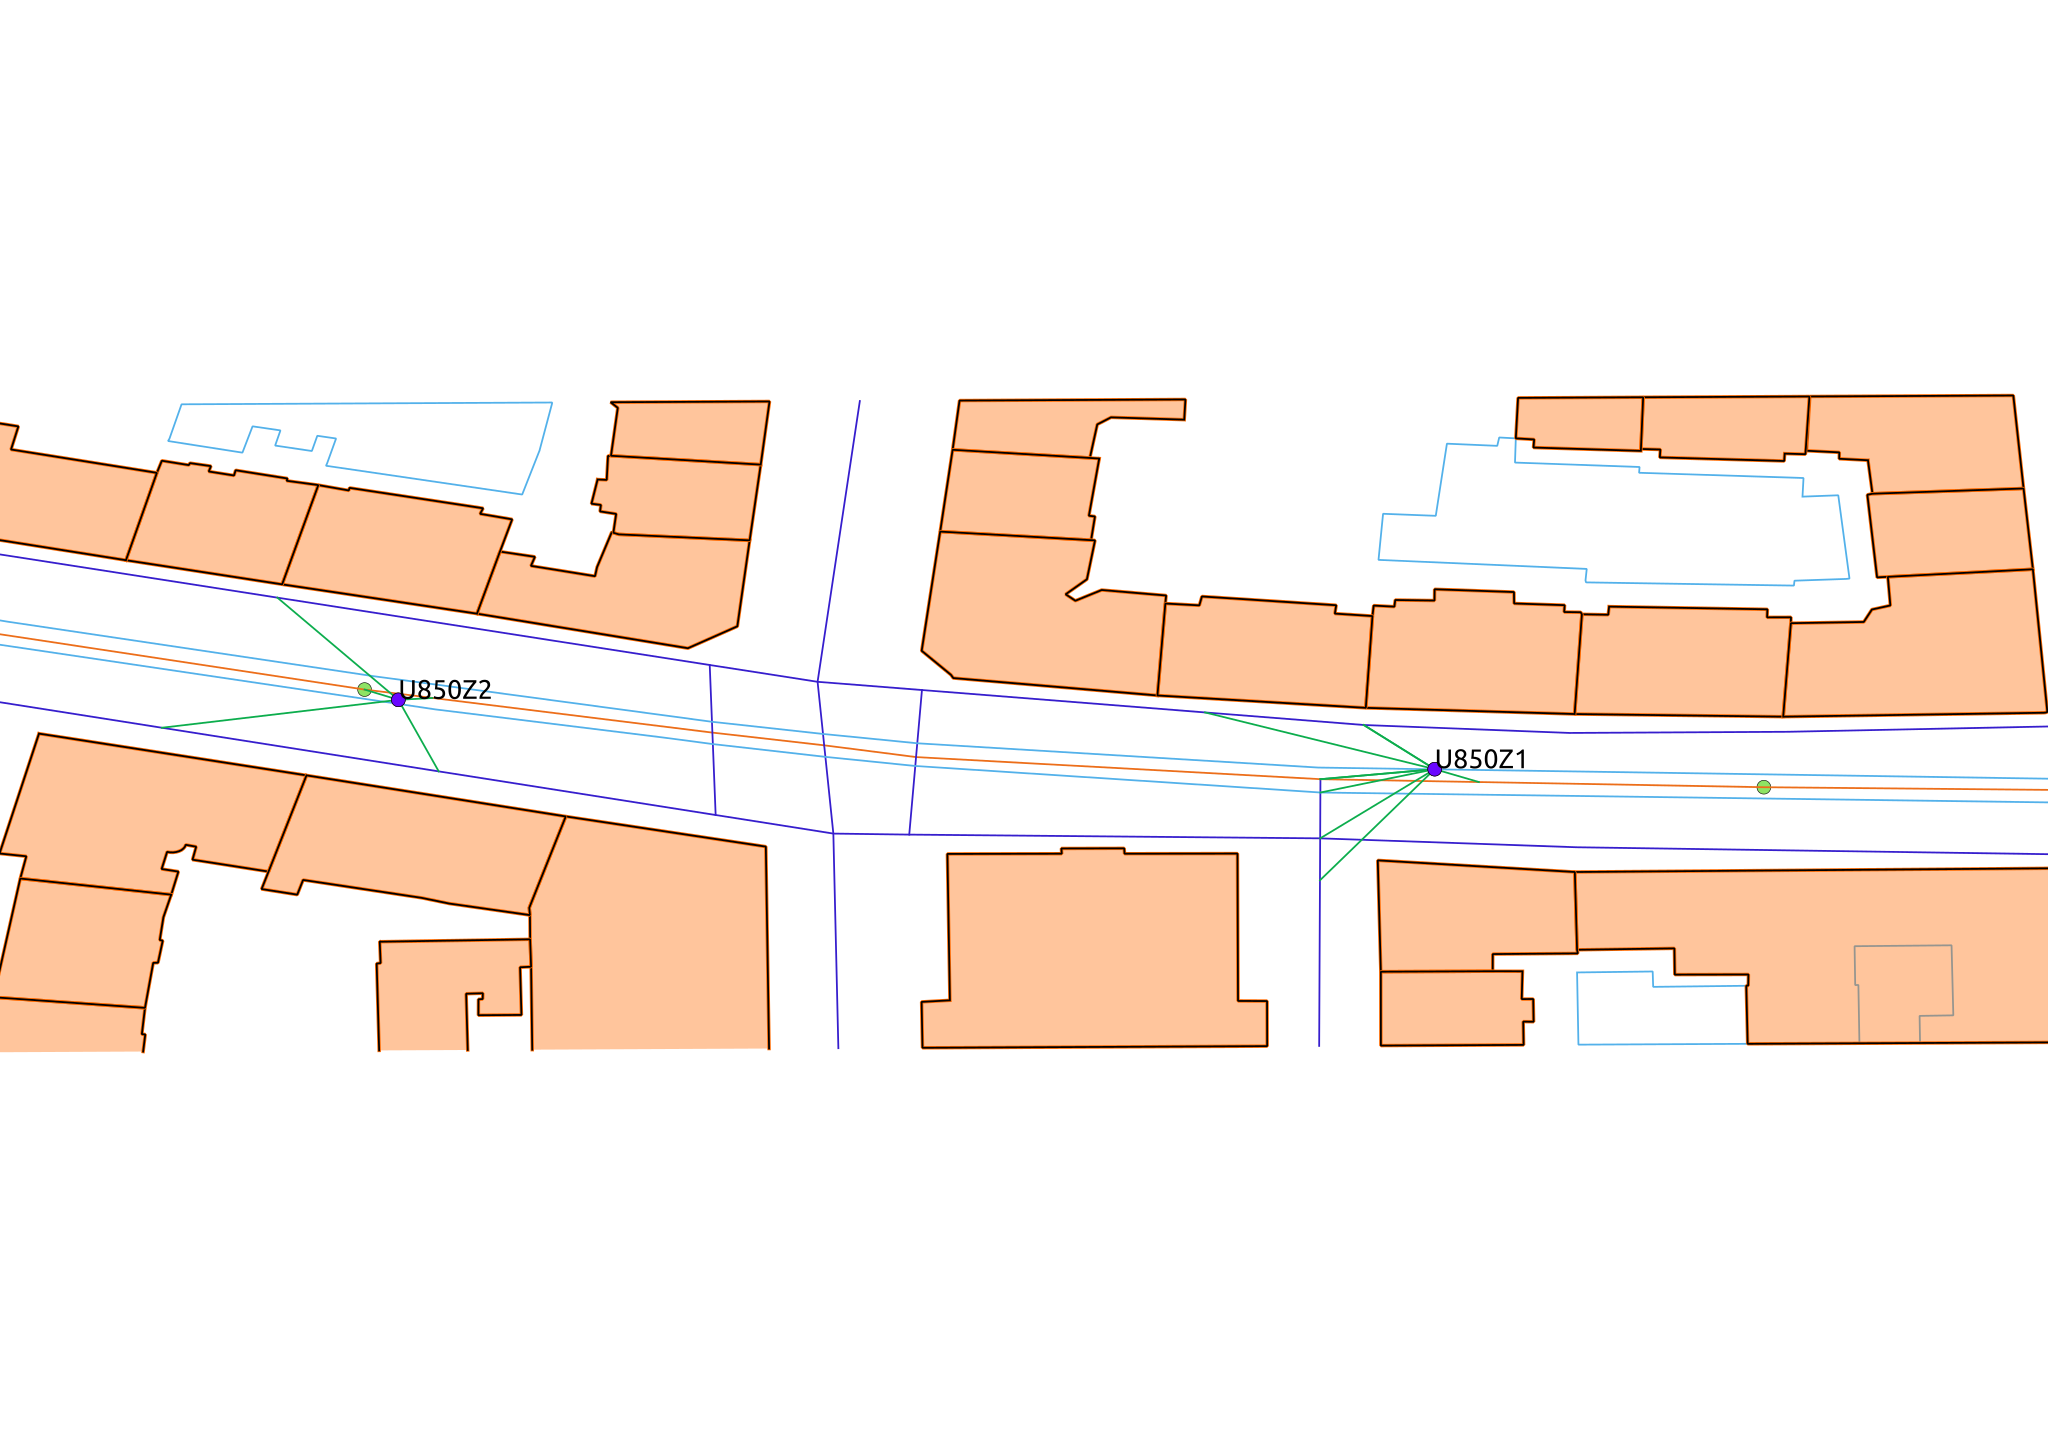
\includegraphics[width=\textwidth]{../img/tramvaj.pdf}
  \caption{Zkratky pro připojení tramvajové zastávky (zeleně)}
  \label{fig:zastavka}
\end{figure}

Pro zastávky z~GTFS, pro které máme v~OSM odpovídající ID, použijeme polohu
z~OSM a zkratky k~cestní síti hledáme z~této polohy. Zkratky jsou i zde potřeba,
protože dle pravidel OSM \cite{OSM} se zastávka umisťuje na místo, kde zastavuje
vozidlo, což například u~tramvají je bod na kolejích, které ale pro pěší
plánování nepoužíváme, tudíž je potřeba najít vhodný blízký bod v~cestní síti.

Zvláštní pozornost je potřeba věnovat u~párování zastávek metra. V~současné
chvíli je metro v~Praze zmapované dvěma způsoby. První způsob (viz obrázek 
\ref{fig:metro-detail}) je novější a
přesnější, jsou při něm zmapována nástupiště a eskalátorové tunely. Při tomto
podrobném mapování jsou také přidána ID stanic, tudíž je možné stanice jednoduše
spárovat a hledat cestu od hrany nástupiště. Častějším způsobem je ale starší
způsob (viz obrázek \ref{fig:metro-hrube}), kdy je stanice metra pouze bod, od
kterého vede eskalátorový tunel na
povrch. Tento eskalátorový tunel je pouze virtuální spojka, neodpovídá reálné
poloze podzemních tras. Takovéto stanice rovněž nemají přiřazená ID. U~těchto
stanic používáme polohu z~GTFS a zkratky spojující zastávku s~cestní sítí
hledáme do blízkých míst, která jsou v~podzemí, což vede k~poměrně dobré
aproximaci přístupu do metra. Jak bude postupovat mapování stanic metra, bude
tento typ stanic postupně eliminován a dojde ke zpřesnění navigace při
přestupech.

\begin{figure}
  \centering
    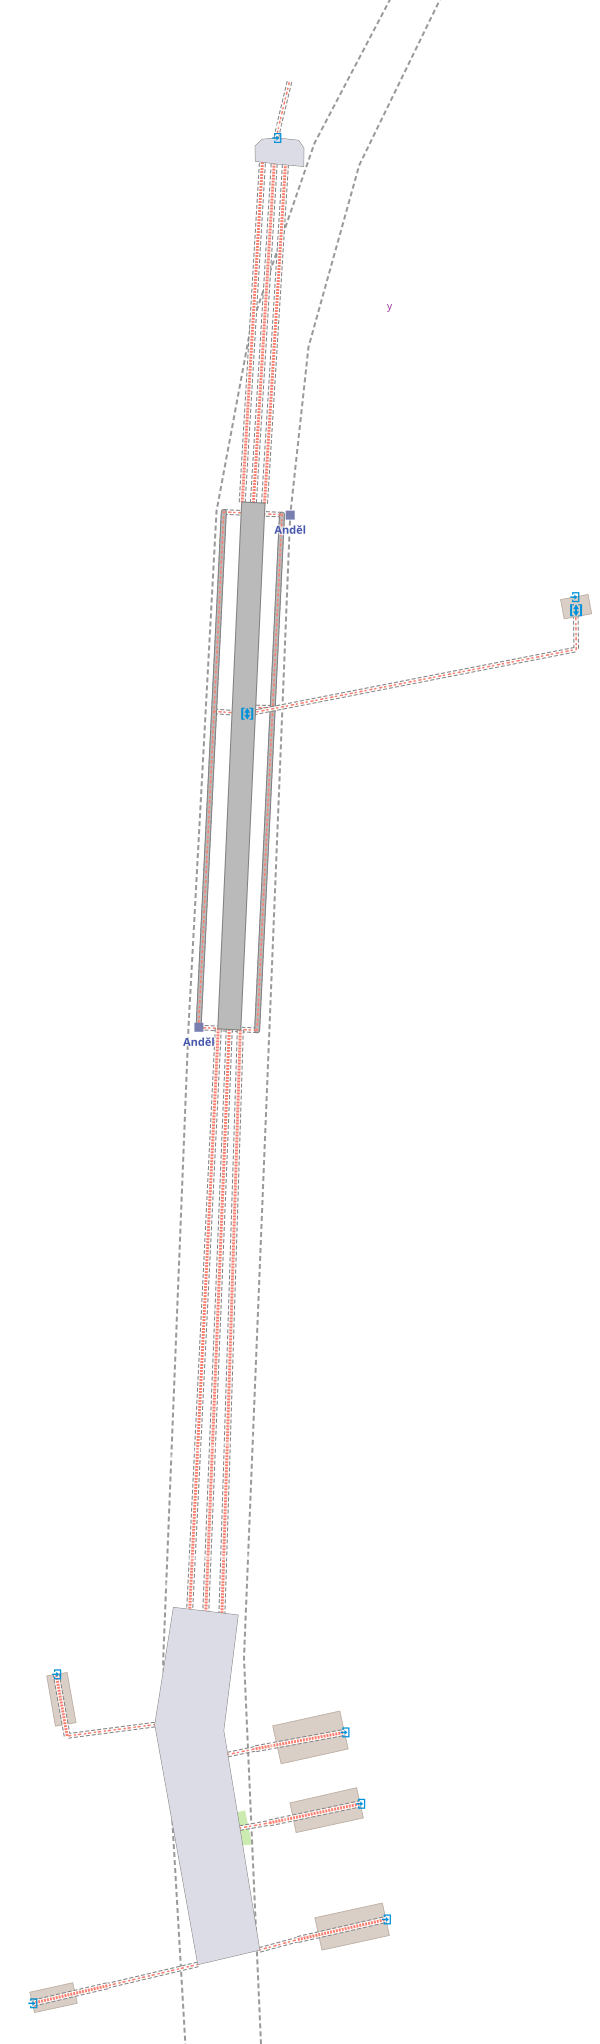
\includegraphics[height=0.99\textheight]{../img/andel.pdf}
  \caption{Detailně zmapovaná stanice metra Anděl}
  \label{fig:metro-detail}
\end{figure}

\begin{figure}
  \centering
    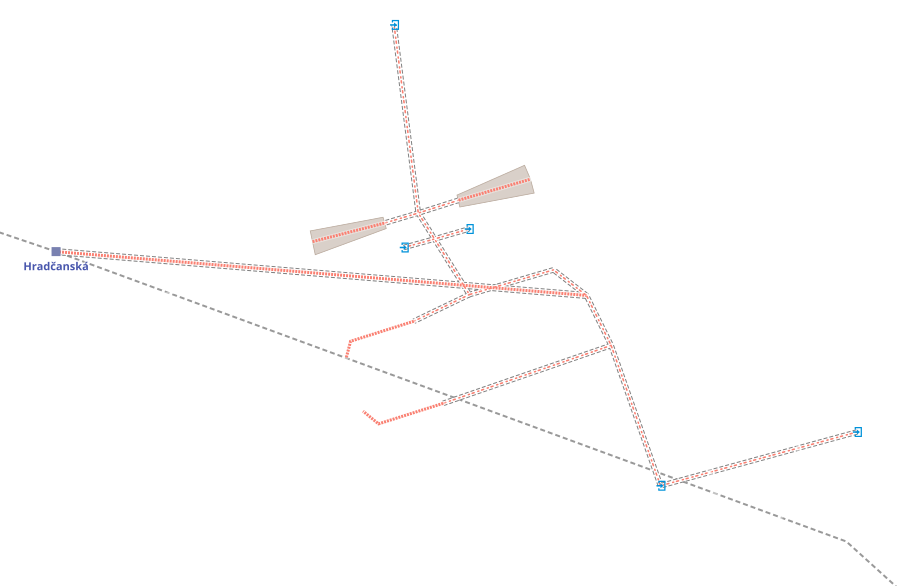
\includegraphics[width=\textwidth]{../img/hradcanska.pdf}
  \caption{Stanice metra Hradčanská zmapovaná starším způsobem}
  \label{fig:metro-hrube}
\end{figure}

Vždy jsou preferovány zastávky a stanice zmapované přesněji, které mají ID,
stačí tedy vylepšovat mapu a při dalším předzpracování dat se nově zmapované
zastávky dostanou i do vyhledávače.


\chapter{Vyhledávání trasy}
    - chodici a mhd hrany
    - funkce na vypocet penalt
    - eliminace duplicitnich tras

\chapter{Implementace}
Pro implementaci programu převádějícího OSM data do formátu vyhledávacího grafu
jsme zvolili v první části Python, protože pro něj existuje široké množství
knihoven, které nám pomohly při řešení jednotlivých dílčích problémů. Při
vytváření spojek mezi cestami a jejich následné kontrole již ale nedostačoval,
proto tuto a další části jsme implementovali v jazyce C. Mezi těmito částmi
předáváme data pomocí Protocol Bufferu v souboru. Vyhledávání je také
implementováno v jazyce C kvůli rychlosti a paměťové nenáročnosti.

\section{Klasifikace OSM dat}
\section{Vyřešení multipolygonů}
\section{Zjednodušení budov}
\section{Rozdělení dlouhých úseků}
\section{Spojky mezi cestami}
\section{Zkratky přes průchozí prostranství}
\section{Vytvoření vyhledávacího grafu}

\chapter{Formáty dat}
V rámci přípravy dat a vyhledávání tras jednak používáme interní struktury
jednotlivých programovacích jazyků, jednak některé standardní formáty nezávislé
na programovacím jazyku. Tyto formáty ppředstvíme v následující sekci, v dalších
sekcích se již jen budeme věnovat obsahu jednotlivých struktur.
\section{Používané formáty dat}
\subsection{Protocol Buffers}
Protocol Buffers (PBF) je způsob uložení strukturovaných dat. Byl navržen
Googlem a je používán v případech, kdy potřebujeme přenést po síti zprávy s
danou strukturou. Formát podoporuje různé datové typy (integer různých přesností
a znaménkovosti, čísla s plovoucí řádovou čárkou, stringy, \dots) a
strukturování zpráv. Komunikace probíhá ve fázích naplnění zprávy, její
zabalení, odeslání, přijmutí a rozbalení. Při zabalení jsou data zkompirmována
jednoduchým algoritmem, aby například malá čísla nezabírala zbytečně mnoho
místa. Existují PBF verze 2 a verze 3. V naší práci používáme verzi 2, protože v
době psaní bakalářské práce, kterou v naší práci rozšiřujeme, nebyly PBF verze 3
ještě k dispozici a verze 3 nepřináší novinky, které by motivovaly k přechodu.

Základní jednotkou PBF je zpráva, která obsahuje několik položek. Položkou může
být základní datový typ nebo jiná zpráva, položky mohou být povinné, volitelné,
nebo opakované. Každá položka má jméno, typ a číslo, které ho identifikuje v
binární podobě zprávy. Zprávy se popisují pomocí vlastního jazyka, ze kterého se
pak pomocí kompilátoru vytvoří vazby do jednotlivých programovacích jazyků. 
Podrobnou dokumentaci včetně tutoriálů lze najít na stránkách projektu (\TODO
ref).

\subsection{JavaScript Object Notation}
JavaScript Object Notation(\TODO ref) (JSON) je formát navržený pro předávání dat ve
webových aplikacích. Díky své jednoduchosti a čitelné reprezentaci je hojně
využíván nejen ve webových projektech, ale často i jako konfigurační jazyk.
Vychází z Javascriptu, datové typy v něm jsou kromě primitivních typů slovník --
neuspořádaný seznam dvojic klíč--hodnota a pole -- uspořádaná posloupnost
položek. Formát zpráv není dopředu dán a podpora v programovacích jazycích je
přímo integrovaná nebo dodaná pomocí knihovny. 

\subsection{GeoJSON}
GeoJSON(\TODO ref) je, jak již název napovídá, nadstavba formátu JSON pro přenos
geografických informací. Z hlediska syntaxe se jedná o korektní JSON, který má
ale předepsanou strukturu a názvy položek. Umožňuje ukládat body, linie, plochy,
multipolygony a další objekty spolu s jejich atributy a je nativně podporován
většinou JavaScriptových knihoven pro zobrazování mapových dat.

\section{Formáty používané při přípravě dat}
\TODO PBF
\section{Formáty používané při vyhledávání tras}
\TODO tt.bin, praha-graph.pbf, JŘ pro konkrétní den, struktury pro hledání,
výstupní PBF, GPX
\section{Formáty používané ve webové aplikaci}
\subsection{Výsledky vyhledávání}
Výsledky vyhledávání jsou předávány z backendu do frontendu webové aplikace
(\TODO ref webová aplikace) pomocí formátu JSON. Ten je tvořen polem vyhledaných
tras, kde každá trasa je slovník s následujícími klíči:
\begin{itemize}
	\item {\tt time} udávající čas příjezdu do cíle
	\item {\tt dist} udávající celkovou pěší vzdálenost na nalezené trase
	\item {\tt penalty} udávající penaltu vyhledané trasy
	\item {\tt geojson} obsahující grafickou reprezentaci nalezené trasy. 
\end{itemize}
Grafická reprezentace nalezené trasy je reprezentována ve formátu GeoJSON a
obsahuje lomené linie jednotlivých typů popisující průběh cesty a bodové prvky
pro nástup a výstup z prostředku MHD.

Liniové prvky (\TODO dopsat) 
\begin{itemize}
	\item	
\end{itemize}
Bodové prvky jsou reprezentovány pomocí typu Point s následujícími atributy: 
\begin{itemize}
	\item {\tt type} udávající typ bodu, zde vždy číslo reprezentující objtype PUBLIC\_TRANSPORT  	
	\item {\tt name} udávající jméno zastávky
	\item {\tt subtype} udávající operaci na zastávce ({\tt departure} pro
	nástup, {\tt arrival} pro výstup)
	\item {\tt departure} čas odjezdu spoje ze zastávky
	\item {\tt arrival} pro nástupní bod čas příchodu na zastávku, pro
	výstupní bod čas příjezdu do zastávky
\end{itemize}
\TODO příklad

\chapter{Uživatelská dokumentace}
\section{Příprava dat}
Pro přípravu dat je nejprve nutné nainstalovat potřebné externí knihovny (viz
soubor {\tt Install}) do
systému nebo do adresáře {\tt ext-lib}. Poté je nutné zkompilovat všechny zdrojové
kódy zavoláním {\tt make} v~adresáři {\tt compiled}. Dále je nutné vytvořit databáze
pro přípravu dat. Pro mapová data je potřeba vytvořit databázi {\tt
osmawalk-prepare},
pro jízdní řády je potřeba vytvořit databázi {\tt gtfs\_praha}. Pak je již možné
přistoupit k~samotné přípravě dat. Pokud je vše správně nastavené, stačí spustit
skript {\tt prepare.sh} v~kořenovém adresáři projektu a po několika hodinách
budou data připravena. Pokud skript selže, dále popíšeme činnosti, které skript
provádí, aby bylo možné jednotlivé fáze spouštět ručně a hledat, kde nastala chyba.

\begin{enumerate}
\item {\tt osm/prepare.sh} slouží ke stažení dat OSM, SRTM, spojení jednotlivých
dílů dat SRTM a tvorbu výřezu z~dat OSM. Výstupem je soubor {\tt osm/praha.osm}
s~výřezem z~dat OSM a soubor {\tt heights.bin} se spojenými daty SRTM pro daný
výřez. 
\item {\tt compiled/parse} slouží ke klasifikaci dat OSM, určení typů objektů,
určení vrcholů na mostech a pod zemí a přiřazení nadmořské výšky k~uzlům.
Výstupem jsou soubory {\tt data/nodes-stage1}, {\tt data/ways-stage1} a {\tt
data/mp-stage1} s~jednotlivými objekty. Formát uložení je popsán v~sekci Formáty
dat\ref{ch:formaty:priprava}. Nastavení klasifikátoru je v souboru {\tt
config/waytypes.yaml} pro cesty a {\tt config/nodetypes.yaml} pro body. Formát
konfiguračních souborů je popsán v bakalářské práci \cite{bakalarka}.
\item {\tt todb.sh} slouží k~nahrání klasifikovaných dat do databáze. 
\item {\tt postgis/process.sh} řídí úpravy dat v~databázi, uvnitř obsahuje
volání jednotlivých kroků popsaných v~kapitole \ref{ch:implementace}.
Výstupem jsou soubory {\tt data/\dots.csv} obsahující vrcholy a hrany dat
připravených pro vyhledávání. 
\item {\tt compiled/csvtograph} Vytváří vyhledávací graf a vybírá v~něm největší
souvislou komponentu, kterou uloží pro hledání jako soubor {\tt
data/postgis-graph.pbf}.
\end{enumerate}

Pro přípravu jízdních řádů stačí v adresáři {\tt ext-lib/mmpf/raptor} spustit
skript {\tt update-gtfs.sh}. Tento skript stáhne aktuální jízdní řády, nahraje
je do databáze a spustí skript {\tt prepare.py}, který připraví soubor {\tt
tt.bin} s jízdními řády. 

Při přípravě dat je potřeba vždy nejprve aktualizovat jízdní řády a pak teprve
aktualizovat mapu. Při přípravě mapových dat dochází i k párování zastávek MHD a
je proto potřeba již mít vygenerované soubory sloužící ke spojení obou datových
souborů.

\section{Konfigurační soubor}
Pro konfiguraci vyhledávání slouží soubor {\tt config/speeds.yaml}. Tento soubor
má formát YAML a skládá se z několika úrovní asociativních polí. Kořenové pole
obsahuje jako klíče jednotlivé kategorie, které jsou nastavovány a jako hodnoty
buď přímo nastavení, nebo další mapování uchovávající nastavení. Kategorie
nastavení jsou následující:
\begin{itemize}
	\item {\tt speeds} udává absolutní rychlosti pěších přesunů. Hodnotou je mapování
	typ cesty $\rightarrow$ rychlost v km/h.
	\item {\tt ratios} udává rychlosti pěších přesunů jako násobek rychlosti
	pohybu po cestě typu {\tt WAY}. Hodnotou je stejné mapování jako u {\tt
	speeds} V případě, že je definována rychlost obojím způsobem, má
	přednost absolutní rychlost před poměrnou.
	\item {\tt penalties} udává penaltu za jednotlivé druhy cest. Hodnotou
	je mapování typ cesty $\rightarrow$ penalta. Penalta se násobí počtem
	sekund strávených procházením hrany. 
	\item {\tt heights} udává koeficient délkového prodloužení v závislosti
	na změně výšky. Hodnotou je mapování s klíči {\tt upscale} a {\tt
	downscale}.  Pokud je cesta do kopce, je prodloužena o {\tt <rozdíl
	výšky>}$\times${\tt upscale} metrů, pokud je z kopce, o {\tt <rozdíl
	výšky>}$\times${\tt downscale}. Cesta může být i zkrácena, pokud by
	celková délka byla záporná, je uvažována jako nulová.
	\item {\tt pt-time-penalties} udává penalty za typ dopravního prostředku
	násobené dobou strávenou v dopravním prostředku v sekundách. Hodnotou je
	mapování typ prostředku $\rightarrow$ penalta, kde typ prostředku je brán
	z GTFS a psán malými písmeny, např. {\tt tram}, {\tt ferry} nebo {\tt
	bus}.
	\item {\tt pt-fixes-penalties} udává fixní penalty za typ dopravního
	prostředku. Počítá se pro každou cestu daným typem prostředku jednou
	nezávisle na délce cesty. Hodnotou je stejné mapování jako u {\tt
	pt-time-penalties}.
	\item {\tt line-penalties} udává penaltu za použití dané linky. Penalta
	se počítá jednou za každé použití dané linky. Hodnotou je mapování jméno
	linky $\rightarrow$ penalta. 
	\item {\tt max-vehicles} udává maximální počet spojů MHD použitých po
	cestě. Hodnotou je číslo udávající tento počet.
	\item {\tt geton-penalty} udává penaltu za nástup do spoje MHD. Je to
	fixní penalta za každý nástup. Hodnotou je číslo udávají penaltu.
	\item {\tt min-wait} udává minimální čas od příchodu /
	příjezdu na zastávku do odjezdu spoje. Hodnotou je čas v sekundách.
\end{itemize}
U kategorií, které udávají penaltu, lze místo čísla napsat {\tt inf}, což znamená
nekonečnou penaltu, tedy pokud nějaké částečná trasa dostane takovouto penaltu,
tak už se dále nepokračuje ve vyhledávání zbytku trasy.

\section{Konzolová aplikace}
Konzolová aplikace slouží převážně pro testování, zda vyhledávací knihovna
pracuje stabilně, ale dá se použít i pro jednoduché hledání. Aplikaci spustíme
v~adresáři compiled příkazem {\tt ./search <flat> <flon> <tlat> <tlon> [time]},
kde {\tt flat} a {\tt flon} určují zeměpisnou šířku a délku výchozího bodu, {\tt
tlat} a {\tt tlon} souřadnice cílového bodu a {\tt time} unixový timestamp času,
od kterého hledat. Pokud není čas uveden, hledá se od
okamžiku spuštění.  Aplikace najde trasy a na standardní výstup vypíše ke každé
trase použité spoje MHD. Navíc v~aktuálním adresáři vytvoří soubor {\tt
track.gpx}, který obsahuje jednotlivé nalezené trasy.
 
\section{Webová aplikace}
Webovou aplikaci je možné vyzkoušet na \url{http://mhd.bezva.org} nebo si ji spustit lokálně
pomocí příkazu {\tt python wsgi.py} v~adresáři {\tt webapp}. V~případě, že knihovna
{\tt libraptor.so} není umístěná tam, kde systém hledá sdílené knihovny, je potřeba ji
do této cesty buď přesunout, nebo zavolat příkaz {\tt export
LD\_LIBRARY\_PATH=<cesta k~libraptor.so>}. Po spuštění aplikace je možné si
otevřít prohlížeč na stránce, která se vypíše během spouštění aplikace.
I~v~případě, že spouštíme aplikaci lokálně, je potřeba mít k~dispozici připojení
k~internetu, protože mapové podklady a javascriptové knihovny se načítají ze
serverů třetích stran.

Po otevření webové aplikace je zobrazené hlavní okno s~mapou. Interakce s~mapou,
kromě základního posouvání a zvětšování, probíhá kliknutím na bod. Prvním
kliknutím je zvolen výchozí bod, ze kterého hledat, druhým kliknutím je zvolen
cílový bod do kterého se hledá trasa. Volbou cílového bodu je odeslán požadavek
na vyhledání trasy. Po vyhledání jsou v~levém sloupci zobrazená shrnutí
jednotlivých nalezených tras v~pořadí podle času příjezdu do cíle a první trasa
je zobrazena v~mapě. Zobrazení nebo skrytí jednotlivých tras se provede
kliknutím na její souhrn v~levém sloupci. Jednotlivé části trasy jsou obarveny
podle typů hran, po kterých vedou a dále jsou zvýrazněna místa přestupu na MHD.
Detailní informace o~MHD lze zobrazit kliknutím na ikonu u~přestupní zastávky
nebo na hranu spoje MHD. Trasy lze exportovat do GPX kliknutím na tlačítko
\uv{Stáhnout jako GPX} v hlavičce stránky.

\section{Výsledky}
- vysledky
  - porovnani s existujicimi vyhledavaci
  - ukazky vyhod vlastnich penalt
  - co s rychlosti

\chapter{Závěr}

\section{Zhodnocení}
Úlohou práce bylo zpracovat veřejně dostupná mapová data a data o~jízdních
řádech a vytvořit z~nich formát vhodný pro vyhledávání spojení kombinujících
pěší přesuny a přesuny hromadnou dopravou. Součástí práce měl být také
vyhledávač, který bude umožňovat nad připravenými daty vyhledávat spojení a bude
možné ho parametrizovat.

Cíl práce se nám podařilo splnit, pro práci s~mapovými daty jsme využili
dřívější bakalářskou práci, kterou jsme dále rozšířili a datový formát
připravili na propojení s~daty z~jízdních řádů. Pro ukládání dat z~jízdních
řádů jsme navrhli formát vycházející z~potřeb algoritmu RAPTOR pro hledání
v~sítích hromadné dopravy. Připravili jsme skripty pro automatický převod dat
jízdních řádů do našeho formátu a implementovali algoritmus RAPTOR jako sdílenou
knihovnu, kterou je možné použít v~jiných projektech nezávisle na zbytku naší
práce. 

Provázali jsme data z~jízdních řádů s~mapovými daty a vypořádali jsme se
s~různou kvalitou zmapování zastávek veřejné dopravy v~mapě. Nad výslednými daty
jsme pak implementovali vyhledávač spojení, který je možné používat jako
sdílenou knihovnu nebo konzolovou či webovou aplikaci. Navrhli jsme systém
hodnocení nalezených tras pomocí penalt a umožnili jsme uživatelům snadno
nastavovat různé penalty pomocí konfiguračního souboru. 

\section{Výsledky}
Spojení nalezená naším vyhledávačem jsou plně srovnatelná se spojeními
nalezenými současnými vyhledávači spojení a na rozdíl od nich můžeme zároveň
využívat možnosti plánovat kvalitní pěší přesuny a nastavovat si parametry
vyhledávače dle svých požadavků. Problémem zůstává nízká rychlost vyhledávání
spojení, víme však, na která místa se zaměřit v~dalších optimalizacích. Návrh
aplikace a převedení přípravy dat do PostgreSQL se osvědčilo a umožnilo snadnou
kontrolu výstupních dat pomocí geografického informačního systému. Rozdělení
přípravy dat do modulů a možnost živého náhledu na zpracovávaná data výrazně
zrychlilo a usnadnilo vyhledávání a odstraňování chyb.

\section{Náměty pro další rozvoj}
Aplikace je v~současné době plně použitelná pro hledání spojení lokálním
uživatelem. Pro použití jako serverová aplikace by kromě zrychlení vyhledávání
bylo nutné i připravit pro uživatele možnost nahrát si vlastní vyhledávací
profily a na straně knihovny se naučit sdílet neměnná mapová data a jízdní řády
mezi více vlákny pro úsporu paměti. 

Zajímavou možností by také bylo upravit vyhledávač do podoby webové aplikace,
optimálně i s~offline daty, a to buď jako samostatnou aplikaci, nebo jako plugin
do některé ze současných mapových aplikací, například OsmAnd.

\subsection{Příprava dat}
Příprava mapových dat je již odladěný proces, který je rychlý a nenáročný na
operační paměť, případné změny by tudíž mířily k~dalšímu vylepšování
připravovaných dat. Jednou z~možností, jak již bylo naznačeno v~kapitole
\ref{ch:vysledky}, by bylo zkoumat okolí cest a mít u~hran v~grafu uložen typ
okolí -- jestli se nacházíme uvnitř zástavby, v~parku či u~velké silnice. Mohly
by tak být penalizovány trasy podle \uv{krásy}.

Přípravu dat jízdních řádů by bylo vhodné přepsat buď jako databázovou aplikaci,
když svá data stejně bere z~databáze, nebo jako samostatnou aplikaci
v~kompilovaném jazyce, která by byla paměťově úspornější. Do výstupního formátu
jízdních řádů by bylo vhodné přidat různé atributy, které se obvykle u~spojů
vyskytují: nízkopodlažnost vozidla, název konečné a další informace, které by
uživatelům usnadnily cestování.

\subsection{Zrychlení vyhledávání}
Pro jiné než lokální použití na počítači je nutné zrychlit vyhledávač spojení.
Zrychlovat vyhledávání je v~současné době možné jak úpravou kódu na
efektivnější, tak změnami v~samotném vyhledávacím algoritmu. Jako první se
nabízí třídit položky u~jednotlivých vrcholů, aby bylo možné majorizace hledat
binárním vyhledáváním místo průchodu celým polem. Z~principu majorizace totiž
u~položek setříděných podle času vzestupně klesá penalta, protože v~opačném
případě by položka s~větším časem a penaltou byla majorizována. Tento přístup by
přinesl složitost do přidávání nových položek, ale zrychlil by rozhodování, zda
položku budeme vůbec přidávat. 

Další možnost zrychlení je přímo ve vyhledávacím algoritmu, kdy můžeme zkoušet
různé jiné typy hald či se pomocí vhodné heuristiky snažit hledat více směrem
k~cíli, jak je uvedeno v~\cite{mj-ga}.

\subsection{Vylepšení vyhledávání}
Mimo zrychlení jsme během práce narazili na různé možnosti, jak zlepšit kvalitu
vyhledávání. Koncept majorizovaných spojení, jak jsme ho navrhli, dává poměrně
dobré výsledky, ale může se snadno stát, že dojde k~majorizaci některých
spojení, které bychom chtěli zachovat. Typická situace je několik možných
začátků trasy, které všechny vedou na stejný spoj. U~nástupního vrcholu do
tohoto spoje se pak sejde několik částečných tras a z~principu penalt bude dále
pokračovat jen jeden z~nich a to ten s~nejmenší penaltou a ostatní se zahodí,
protože mají všechny stejný čas odjezdu. Možným řešením je nemajorizovat jinou
částečnou trasu, která se liší použitými spoji, bylo by však potřeba zjistit,
zda pak vyhledaných spojení nebude příliš mnoho.  

Obdobným problémem je preference častějších spojení, kdy bývá výhodné jít na
zastávku, odkud jezdí spoje často a případný ujetý nebo zpožděný spoj nám
nezkazí celý zbytek cesty. K~tomuto problému je možné přistupovat dvěma způsoby,
jednak lze pro každou vyhledanou trasu zkoumat alternativy v~případě ujetí
jednotlivých spojů po cestě, jednak lze frekvenci spojení nějakým způsobem
zanést do systému penalt a preferovat tak frekventovanější trasy před ostatními. 

Systém penalt lze rozšiřovat mnoha dalšími způsoby, například zavést směrové
penalty. Mezi takové by mohla patřit penalta za chůzi do schodů, ale směrové
penalty dávají smysl u~spojů MHD, kdy poblíž konečné mohou být spoje směrem na
konečnou často zpožděné, zatímco spoje z~konečné bývají spolehlivé a jedou včas.
Dalším vylepšením penaltového systému by byla konfigurace pomocí vhodného
skriptovacího jazyka na místo konfiguračního souboru, kdy by bylo možné si
výpočet penalt přizpůsobit přesně podle svých potřeb a nebylo by pak potřeba
znovu překládat celý program. Tato úprava by ale mohla mít negativní dopad na
rychlost vyhledávání.

Kombinované vyhledávání pěších tras s~přesuny hromadnou dopravou má ještě jedno
specifikum a tím je čas nutného odchodu z~výchozího místa. Pokud jdeme několik
stovek metrů na autobus, který jezdí jednou za půl hodiny, pak není třeba
vycházet hned po nalezení spoje, ale stačí nám vyjít například až za 10 minut a
do cíle dorazíme ve stejný čas. Tato situace je řešitelná poměrně snadno
posunutím pěší části trasy před prvním přejezdem MHD tak, aby pěší trasa na spoj
MHD akorát navazovala. Problém je ale obecnější, pokud autobus s~půlhodinovým
intervalem používáme až na konci cesty, pak nestačí jen posunout první pěší
část, ale mohli bychom jet i pozdější tramvají a tudíž by bylo potřeba i změnit
některé spoje na trase či celou část trasy. Problém se dá (neefektivně) řešit
postupným hledáním v~pozdějších časech, pokud na cestě narazíme na spoj
s~velkým intervalem, ale pro efektivnější řešení by bylo potřeba nastudovat
potřebnou literaturu, provést měření a pravděpodobně by se jednalo o~velký zásah
do vyhledávacího algoritmu.


%%% Seznam použité literatury
\begin{thebibliography}{10}

\bibitem{time-expanded}
	{\sc Pyrga} Evangelia a kol.
	\emph{Efficient models for timetable information in public
	transportation}.
	J. Exp. Algorithmics. 12:2.4:1--2.4:39. 2008-06.

\bibitem{time-dependent}
	{\sc Gerth~Stølting} Brodal, {\sc Riko} Jacob.
	\emph{Time-dependent networks as models to achieve fast exact
	time-table queries}. 
	Electronic Notes in Theoretical Computer Science.
	92:3 -- 15. 2004.

\bibitem{CH}
	{\sc Geisberger}, Robert.
	\emph{Contraction of timetable networks with realistic transfers}.
	CoRR.
	abs/0908.1528. 2009.

\bibitem{RAPTOR}
	{\sc Delling}, Daniel, {\sc Pajor} Thomas, {\sc Werneck} Renato~F.
	\emph{Round-based public transit routing.}
	Transportation Science.
	49(3):591--604. 2015.

\bibitem{OSM}
	{\sc přispěvatelé OSM}.
	\emph{OpenStreetMap} [online]
	2017 [cit. 2017-07-15].\\
	Dostupné z~\url{http://www.openstreetmap.org/about}

\bibitem{bakalarka}
	{\sc Pokorný}, Tomáš.
	\emph{Hledání pěších cest v~mapě}.
	Praha, 
	2014.
	Bakalářská práce. Matematicko-fyzikální fakulta, Katerda aplikované
	matematiky.

\bibitem{SRTM}
	{\sc National Aeronautics and Space Administration.}
	\emph{The Shuttle Radar Topography Mission} [online]. 
	2009-06-17 [cit. 2014-05-04]. \\
	Dostupné z: \url{http://www2.jpl.nasa.gov/srtm/}.

\bibitem{GTFS}
	{\sc Google.}
	\emph{General Transit Feed Specification} [online]. 
	2017 [cit. 2017-07-15]. \\
	Dostupné z: \url{https://developers.google.com/transit/gtfs/reference/}.

\bibitem{PBF}
	{\sc Google.}
	\emph{Protocol Buffers} [online]. 
	2012-04-02 [cit. 2014-05-05]. \\
	Dostupné z: \url{https://developers.google.com/protocol-buffers/}.

\bibitem{JSON}
	{\sc ECMA}.
	\emph{The {JSON} data interchange format} [online].
	Technical Report Standard ECMA-404 1st Edition.
	2013-10 [cit. 2017-07-15].\\
	Dostupné z:
	\url{http://www.ecma-international.org/publications/files/ECMA-ST/ECMA-404.pdf}

\bibitem{GeoJSON}
	{\sc Butler}, H. {\sc Daly}, M. a kol.
	\emph{The GeoJSON format} [online].
	RFC 7946.
	2016-08 [cit. 2017-07-15].
	Dostupné z: \url{https://tools.ietf.org/html/rfc7946}

\bibitem{XML}
	{\sc Bray}, Tim. {\sc Paoli}, Jean a kol.
	{\em Extensible Markup Language (XML) 1.0 (Fifth Edition)} [online].
	W3C.
	2008 [cit. 2017-07-15].
	Dostupné z:
	\url{http://www.w3.org/TR/REC-xml/}

\bibitem{GPX}
	\emph{GPX: the GPS Exchange Format} [online]. 
	2017 [cit. 2017-07-15].\\ 
	Dostupné z: \url{http://www.topografix.com/gpx.asp}

\bibitem{WGS84}
	{\sc National Imagery and Mapping Agency.}
	\emph{World geodetic system 1984} [online]. 
	3. vydání, 1. dodatek.
	2000-01-03 [cit. 2017-07-15]. \\
	Dostupné z: \url{http://earth-info.nga.mil/GandG/publications/tr8350.2/wgs84fin.pdf}.

\bibitem{UTM}
	{\sc Hager} JW, {\sc Behensky} JF, {\sc Drew} BW.
	\emph{The universal grids: Universal Transverse Mercator (UTM) and Universal 
	Polar Stereographic (UPS)} [online].
	Tech. Rep. TM 8358.2, Defense Mapping Agency.
	1989, [cit. 2017-07-15].\\
	Dostupné z: \url{http://earth-info.nga.mil/GandG/publications/tm8358.2/TM8358_2.pdf}.

\bibitem{LibUCW}
	{\sc Mareš}, Martin a kol.
	\emph{LibUCW} [online].
	2016 [cit. 2017-07-15].\\
	Dostupné z: \url{https://www.ucw.cz/libucw/}	

\bibitem{Flask}
	\emph{Flask Documentation} [online].
	2017. [cit. 2017-07-15].\\
	Dostupné z: \url{http://flask.pocoo.org/docs}

\bibitem{mj-ga}
	{\sc Mareš}, Martin.
	\emph{Krajinou grafových algoritmů}. [online]
	ITI Series.
	2007 [cit. 2017-07-15].\\
	Dostupné z: \url{http://mj.ucw.cz/vyuka/ga/}

\end{thebibliography}


%%% Obrázky v diplomové práci
%%% (pokud jich je malé množství, obvykle není třeba seznam uvádět)
%\listoffigures

%%% Tabulky v diplomové práci (opět nemusí být nutné uvádět)
%%% U matematických prací může být lepší přemístit seznam tabulek na začátek práce.
%\listoftables

%%% Použité zkratky v diplomové práci (opět nemusí být nutné uvádět)
%%% U matematických prací může být lepší přemístit seznam zkratek na začátek práce.
\chapwithtoc{Seznam použitých zkratek}
\begin{tabular}{ll}
GTFS& General Transit Feed Specification\\
SRTM& Shuttle Radar Topography Mission\\
MHD& Městská hromadná doprava\\
GPX& GPS exchange format\\
XML& Extensible Markup Language\\
PBF& Protocol Buffer\\
OSM& OpenStreetMap\\
\end{tabular}



%%% Přílohy k diplomové práci, existují-li. Každá příloha musí být alespoň jednou
%%% odkazována z vlastního textu práce. Přílohy se číslují.
%%%
%%% Do tištěné verze se spíše hodí přílohy, které lze číst a prohlížet (dodatečné
%%% tabulky a grafy, různé textové doplňky, ukázky výstupů z počítačových programů,
%%% apod.). Do elektronické verze se hodí přílohy, které budou spíše používány
%%% v elektronické podobě než čteny (zdrojové kódy programů, datové soubory,
%%% interaktivní grafy apod.). Elektronické přílohy se nahrávají do SISu a lze
%%% je také do práce vložit na CD/DVD. Povolené formáty souborů specifikuje
%%% opatření rektora č. 13/2017.
\appendix
\chapter*{Příloha B}
\addcontentsline{toc}{chapter}{Příloha B}
V této příloze popíšeme adresářovou strukturu na CD.
\begin{itemize}
	\item \verb|QOsmWalk/| -- Grafická nadstavba vyhledávače tras
	\item \verb|compiled/| -- zdrojové kódy programů v C pro přípravu dat a vyhledávání tras
	\item \verb|config/| -- soubory s nastavením pro klasifikaci a vyhledávání
	\item \verb|data/| -- složka obsahující ProtocolBuffer soubory
	\item \verb|osm/| -- soubory a programy pro stažení a předpřípravu OSM a SRTM dat
	\item \verb|scripts/| -- skripty pro přípravu dat v Pythonu 
	\item \verb|text/| -- zdrojové kódy tohoto textu
\end{itemize}



\openright
\end{document}
